\documentclass[conference]{IEEEtran}
\IEEEoverridecommandlockouts
% The preceding line is only needed to identify funding in the first footnote. If that is unneeded, please comment it out.
\usepackage{cite}
\usepackage{amsmath,amssymb,amsfonts}
\usepackage{algorithmic}
\usepackage{graphicx}
\usepackage{textcomp}
\usepackage{xcolor}
\def\BibTeX{{\rm B\kern-.05em{\sc i\kern-.025em b}\kern-.08em
    T\kern-.1667em\lower.7ex\hbox{E}\kern-.125emX}}
\begin{document}
\\
\\
\title{Vehicle Routing problem }

\author{\IEEEauthorblockN{Keval Savaliya}
\IEEEauthorblockA{\textit{BTech - ICT} \\
\textit{DAIICT}\\
Gandhinagar, India\\
\qquad 201901006@daiict.ac.in \qquad}
\and

\IEEEauthorblockN{Arik Dholiya}
\IEEEauthorblockA{\textit{BTech - ICT} \\
\textit{DAIICT}\\
Gandhinagar, India\\
\qquad 201901009@daiict.ac.in \qquad }
\and

\IEEEauthorblockN{Sanny Dhameliya}
\IEEEauthorblockA{\textit{BTech - ICT} \\
\textit{DAIICT}\\
Gandhinagar, India  \\
\quad 201901031@daiict.ac.in \quad }

\and
{\IEEEauthorblockN{Purav Kansara}
\IEEEauthorblockA{\textit{BTech - ICT} \\
\textit{DAIICT}\\
Gandhinagar, India \\
\qquad 201901032@daiict.ac.in \qquad }
\and

\IEEEauthorblockN{Abhi Dholiya}
\IEEEauthorblockA{\textit{BTech - ICT}  \\
\textit{DAIICT}\\
Gandhinagar, India  \\
\qquad 201901069@daiict.ac.in \qquad } 
\and

\IEEEauthorblockN{Aditya Ramanuj}
\IEEEauthorblockA{\textit{BTech - ICT} \\
\textit{DAIICT}\\
Gandhinagar, India \\
\qquad 201901138@daiict.ac.in \qquad }
 }
}

\maketitle

{\section{\textbf{Abstract}}}
Distribution companies face greater challenges in organizing their fleets efficiently. So they solve the problem by using VRT. The vehicle routing problem is a combinatorial optimization problem. The optimal set of routes for a group of vehicles to traverse is used to deliver to a given set of customers. The VRP has several variants depending on tasks performed and restrictions, such as time windows, multiple vehicles, backhauls, simultaneous delivery, pickup, etc. This paper establishes a model for a large-scale vehicle routing problem with simultaneous pickup and delivery, and the objective is to minimize total transportation costs. The possible preliminary answer is acquired through a miles exceptional transportation efficiency-primarily based on a set of rules and progressed via way of means of a nearby seek set of rules primarily based totally on variable community seek. The computational consequences suggest that the proposed set of regulations computes with the experimental techniques withinside the articles and improves numerous best-acknowledged solutions. \\


{\section{\textbf{Introduction}}}
Physical distribution is one of the key capabilities withinside the logistics industry. A very costly and time-consuming function, especially for the distribution industries, is called a Vehicle routing problem(VRP). Dantzig and Ramser first proposed this problem in 1959 as a generalized problem of traveling salesman problem. Since then, many loads of studies works have been posted on numerous editions of VRP. Vehicle routing problems are beneficial in lots of real-international programs like items distribution, mail delivery, schools bus routing, garbage collections, private travel operations, courier service applications, newspaper distribution, etc. Even though VRP is classed into many editions, the most essential and important variations of VRP are capacitated VRP (CVRP), VRP with time windows (VRPTW), VRP with pickup and delivery (VRPPD), and
 Open VRP (OVRP). The problem taken up in this work is that of a private logistics service provider, who has numerous depots throughout the location with clients spread throughout all of the depots. CVRP with simultaneous pickup and delivery between depots with numerous nodes spread in between them is considered. In this problem, we use VRPPD ( Vehicle Routing Problem with pickup and delivery).
\\



{\section{\textbf{Aim and objective}}}   \\

We prefer the expression VRP with pickups and deliveries (rather than deliveries and pickup) to signify that all goods come from the depot or arrive there. There is no inter-customer transportation of goods. This paper looks at pickup-and delivery problems, where goods are taken directly from one customer to another. While that is a crucial problem, it isn't always an extension to the VRP because it lacks the multi-stop tour planning aspect.  Customers who receive goods from the depot are called linehaul or deliveries; customers who send goods are backhauls or pickups. A customer may also wish to both send and receive goods. This case is called combined demands. If all clients are both natural deliveries or pure pickups, it is called single demands.  Since the seminal paper of Casco, Golden, and Wasil (1988), initially, most VRPDP studies targeted three essential problem classes. The first one is The VRP with Backhauling (VRPB) is a selected case of single demands, constructed on the idea that all deliveries ought to be served before pickups can begin. We provide an explanation for the motivation for this in a few details later on.  \\ 
\\
Second is The VRP with Mixed Deliveries and Pickups (VRPMDP), on the alternative hand, does now no longer make the above assumption and permits deliveries and pickups to arise in any order on a vehicle route. The remaining third one is The VRP with Simultaneous Deliveries and Pickups (VRPSDP) is a case of combined demands in which the vehicle makes a single stop to both deliver and pick up goods. However, this expression also denotes that customers simultaneously have delivery and pickup demand, i.e., a synonym for combined needs. It is profitable to note that the VRPMDP can be modeled as a VRPSDP by including a pickup of zero to every linehaul and delivery of zero to every backhaul. This does not make the model unduly more complicated. However, the VRPSDP can't be modeled as a VRPMDP. One can create fictitious co-placed customers (one purely linehaul one in simple terms backhaul) to transform the problem from combined demands to single demands. However, if this is solved as a VRPMDP, the requirement of a simultaneous visit might not be satisfied.\\


{\section{\textbf{problem statement}}}  
Multiple Travelling Salesman Problems combined with Together which is called The Vehicle Routing Problem. So, now we understand how default solves this problem as opposed to a different NP-complete problem. The goal is not just to find the optimal overall path but also to dynamically find the optimal approach for each vehicle and its deliveries. The purpose of the VRP is to find the optimal approach for each vehicle's route. Our main motto in this project is to solve the problem of some organization or a big transportation company having to transport goods to different locations using different vehicles every day. The problem is that the transportation is very costly and very time-consuming, So the overall efficiency of the delivery system will be reduced. So, using the Vehicle Routing Algorithm, we can achieve our efficiency and Make more Profit. Determining the route can be done by several different methods like time, priority, and demand in the VRT problem. In practice, the basic vehicle routing problem is extended with constraints, for example, on the allowed capacity of the vehicle, length of route, arrival, departure and repair time, time of assortment, and delivery of products. Several variations and specializations of the vehicle routing problem exist. So, We pick up the specific type of problem in the vast VRT problem: the pickup and delivery problem.\\
\\ The pickup and delivery problem (PDP) is a problem of finding a set of optimal routes for a fleet of vehicles to serve a group of transportation requests. Each vehicle from the fleet has a given capacity, a start location, and an end location. Each transportation request is specified by a load to be transported, a source, and a destination location. In other words, the pickup and delivery problem deals with the construction of optimal routes to visit all pickup and delivery locations and satisfy precedence and pairing constraints. Precedence constraints deal with the restriction, in which each pickup location has to be visited before visiting the corresponding delivery location. Pairing constraints restrict the set of admissible routes so that one vehicle has to do both the pickup and the delivery of the load of one transportation request. A review of various approaches to the solution of VRPPD is presented in Desaulniers et al. (2000), Cordeau et al. (2007), and Parragh et al. (2008). So Our main real-life application to solve using this algorithm
is,

\\ \\
“ We are given\textbf{ N }different\textbf{ locations} (here given coordinates of each location ) and \textbf{V} different \textbf{vehicles} (let's suppose given Trucks). For each location ,\textbf{di }is \textbf{demand}  and location is (xi,yi) with their \textbf{pick-up point }\textbf{(xip,yip)} and \textbf{delivery point (xid,yid)}  and the\textbf{ capacity }of each vehicle is \textbf{C}. So, here we want to \textbf{Minimizing the total distance} by each of vehicle to it’s pick-up and delivery locations. The real life application of it is Goods distribution .In this problem,each of vehicle departs from the vehicle depart  they belong to and back the same depot after visiting several locations with a series of loading and unloading operations the objective is to minimizing the trip total cost used to satisfy all delivery requests while meeting loading constraints and time limit. ”
\\
\\
\begin{center}
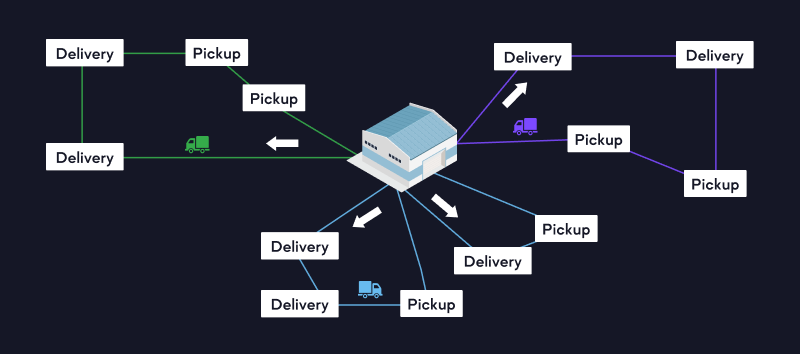
\includegraphics[width=1\linewidth ]{
opt2.png}\par  
\end{center}
\hline
\vspace{5}
\newline
\section{{\textbf{Brief Literature review}}}
\subsection{{\textbf{CAPACITATED VEHICLE ROUTING problem WITH PICK-UP AND ALTERNATIVE DELIVERY(CVRPPAD) : MODEL 
}}}
Various forms of Vehicle Routing Problems occur in the field of product distribution/shipments. Solving these problems within optimum time and costs is becoming a major issue in modern distribution systems. The vehicle routing problem aims to answer the question, "What is the optimal set of routes for a set of vehicles/transportation modes to travel to deliver it to the given set of customers at the appropriate timing." The main objective of VRP is generally to minimize the route cost. The objective functions may vary with the particular application and its variants. But the most common objectives are given below; with the used means of transport (e.g., vehicles) and the distance traveled, we have to minimize all transportation costs associated with it Cover all the given delivery points with the minimum number of transport vehicles available; To minimize the overrun in the situation when estimated travel time and vehicle have been exceeded;\\

\subsection{{\textbf{LITERATURE REVIEW ON THE VEHICLE ROUTING problem IN THE GREEN TRANSPORTATION CONTEXT, Luna Azul  no.42 Manizales Jan./June 2016
}}}
The article explains the importance of transportation in the supply chain. Since the vehicle routing problem's First method in 1959, there have been many courses and has elevated its scope. Initial research had been carried out for analyzing distribution management. Another component that has gained interest is the inclusion of technological improvements in the VRP. About the environment, transportation is one of the most seen within the supply chain aspects. A growing interest is likewise visible by companies to reduce the environmental effect in their products and services (Quariguasi et al., 2009). VRP problems can be classified by developing a taxonomy or developing a generalized framework that summarizes the existing models, the targets pursued and the theories related to the evaluation of the problem (Reisman, 1992). The VRP in its one-of-a-kind forms was initially addressed using actual strategies together with Branch and Bound algorithm proposed through Laporte and Nobert (1987); Fischetti, Toth, and Vigo (1994) and Baldacci and Mingozzi (2004), Branch and Cut taken into consideration through Cordeau (2006), Branch and Price turned into posed by Pessoa et al., 2008; Martinelli et al.,
2011, and Branch and Cut and Price proposed through Baldacci et al. ( 2010).
\\

\subsection{{\textbf{APPROACHES TO SOLVE THE VEHICLE ROUTING problem IN THE VALUABLES DELIVERY DOMAIN : Vladimir Korablev, Ivan Makeev, Evgeny Kharitonov, Boris Tshukin and Ilya Romanov}}}This PDF includes the Description of developed algorithms. The various extensions of the vehicle routing problem with time windows (VRPTW) are considered. In addition to the VRPTW, the authors present a method to solve the SDVRPTW – the version of the project allowing separate objects to be delivered to the customers. The features of this problem solved are additional route restrictions, such as the maximum time, the number of clients and cost, and the most range of vehicles required for delivery. This article is dedicated to valuable delivery problems and strategies to clear them up. The algorithms defined in this text use an evolutionary approach. First of all, the set of solutions (population) is initialized. It is represented schematically. Further, regular development takes region iteratively at the made populations. At a certain iteration, the stop condition is met.\\

\subsection{{\textbf{A SURVEY ON VEHICLE ROUTING problem AND ITS VARIANTS}}}

This paper consists of a literature assessment of the latest tendencies and guides regarding the vehicle routing problem and its variants, specifically vehicle routing problem with time windows (VRPTW) and the capacitated vehicle routing problem (CVRP) and additionally their variants. There are different classes or variations of VRP similar to the capacitated VRP (CVRP), VRP with Time Windows (VRPTW). In the
CVRP, a fleet of identical vehicles positioned at a significant depot, needs to be optimally routed to supply a set of customers with known demands. The goal of the VRPTW is to serve a number of clients inside predefined time windows at minimal cost (in terms of distance traveled) without violating the capacity and total trip time constraints for every vehicle. Exact algorithms to solve VRP, especially the capacitated VRP (CVRP), include the branch-and-bound, the branch-and-cut, and the branch-and-price algorithms.
\\

\section{{\textbf{Current state of art}}}
The problem of vehicle routing is very useful for transportation, but it is very big and complicated. This problem has many several variations, which are divided using different constraints like capacity of the vehicle, length of route, arrival, departure and repair time, time of assortment, and delivery of products. But here we will consider only the problem of Pickup and Deliveries of goods using vehicles and try to minimize the total cost of the trip. In the VRP with Pickup and Delivery(VRPPD), goods must be picked up from a certain location and dropped off at their destination. The pickup and drop-off must be done by the same vehicle, which is why the pickup location and drop-off location must be included in the same route. Hear one of the advanced versions of pickup and delivery. The related problem is the VRP with backhauls where a vehicle does delivery and pickups in one route. Some customers require deliveries and others pickups. We can also add one more constraint in the VRPPD problem with the time window, which is denoted minimum time and minimum cost to get all the tours completed. Recently, some of these variants have been combined into so-called 'Rich' vehicle routing problems, simultaneously including multiple real-life aspects. Let's have some discussion about our current problem and also mathematically define our problem. \\

\begin{center}
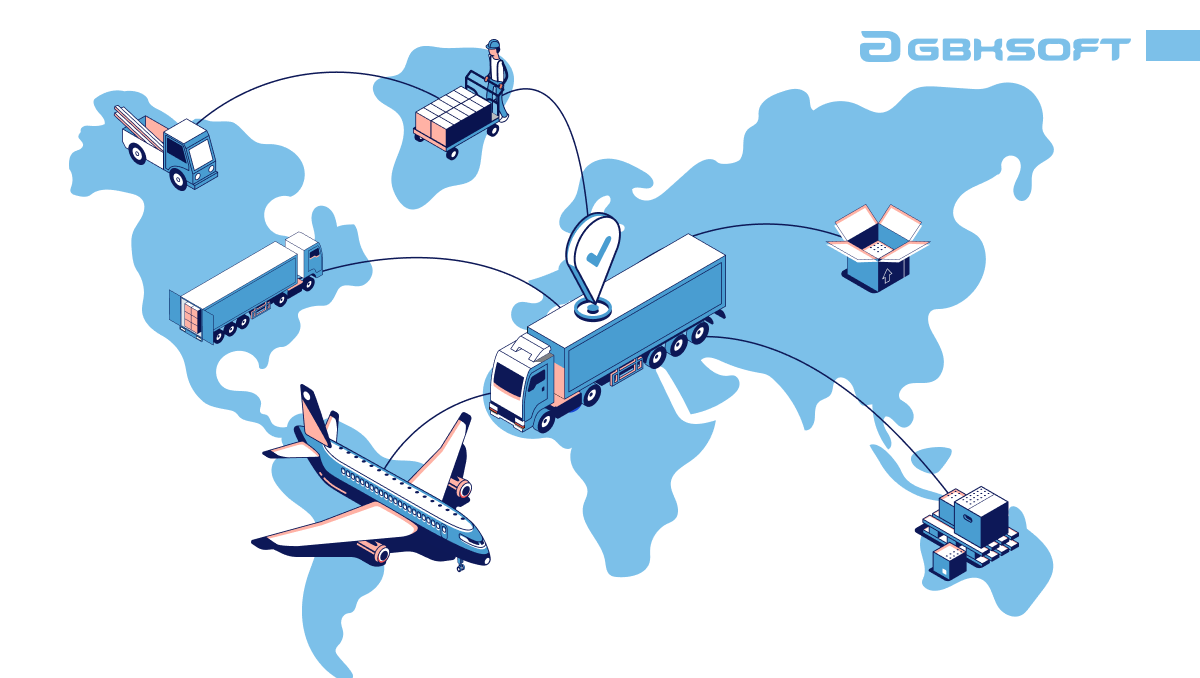
\includegraphics[width=1\linewidth]{
Cover-1.png}\par  
\end{center}

\subsection{{\textbf{problem Description}}}\label{AA}
The problem could be started as follows, there is a set of homogeneous vehicles V={1,2,.....$|V|$}.Each vehicle pick-up and delivery of different kinds of goods to different locations and after they are done working , they go back to the same depot position. Here is given the set of data of N different locations using their (xi,yi) corresponding coordinates.For each of the locations we also gave the demand of goods which denoted using di. Also here given the capacity of each of the trucks is C.Using this information we
will be able to find the different sequences of delivery for Vi vehicle which is denoted by Ti (which is denoted Tour sequences, i-th vehicle travel different location in they current tour.) and try to minimize the trip total cost used to satisfy all delivery requests.hear the total cost which means the distance traveled by vehicle is minimized.\\


\begin{center}
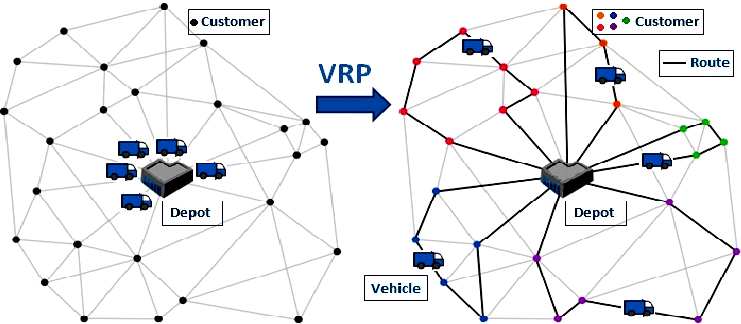
\includegraphics[width=1\linewidth]{
VRT.png}\par  
\end{center}

\vspace{5}

\subsection{{\textbf{Equations}}}\\
\vspace{1}
\begin{enumerate}
\item $|Ti|$ = Length of the current traveled locations sequence of i the vehicle \\ 
\item Vi = denoted i th vehicle \\ 
\item Di = demand of i th location \\
\item xi,yi = coordinate of pick-up or delivery point \\
\item C = capacity of the vehicles \\
\end{enumerate}


$$ Z = \sum\limits_{i \in V}{((dist(0, T(i,0))) + \sum\limits_{(j, k) \in Ti}{dist(j, k)} + }$$ \\$${dist(T(i, |Ti| - 1),0))} $$
Subject to ,

$$  \sum\limits_{j \in Ti}{dj \leq C (i \in V)} $$

Above equation is denoted that the in sequences of i the vehicle sum of all the demand in sequences will less then the capacity of vehicle.

$$  \sum\limits_{i \in V}{(j \in Ti)} = 1 (j \in N / \{0\}) $$

This equation denoted that all the locations are visited using the given vehicles.

\vspace{10}

\section{{\textbf{PLAN OF WORK}}}
\subsection{{\textbf{Goal:1}}}
\subsubsection{{\textbf{Intentions}}}
 Finding good quality and more quantity research paper or reference  material.  Formulating clear abstract and problem statements  \\
\subsubsection{{\textbf{Timeline}}}
16th Sept -  22nd Sept 2021. \\
\subsubsection{{\textbf{Work progress}}}
First of all we decide to find a relevant research paper or any article on our topic. So we all find one or two articles or papers on it. Then we discuss all of our problems . From this paper and articles, we made our problem statement.


\subsection{{\textbf{Goal:2}}}

\subsubsection{{\textbf{Intentions}}}
Understand the theory involved in problem solving about VRP(vehicle routing problem ) and decide the subtopic which this project is about. \\

\subsubsection{{\textbf{Timeline}}} 3rd oct - 11th oct 2021. \\ 
\subsubsection{{\textbf{Work progress}}}
For better understanding of our problem statement and theory behind it, we watched a YouTube video. Now, we know about our problem very well. In this problem we have many variants of VRT. Then we decided to go on with  VRPPD(vehicle routing problem with pick-up and delivery ) nicely. Also we put Video link and research paper or reference link in our reference part.  

\subsection{{\textbf{Goal:3}}}

\subsubsection{{\textbf{Intentions}}}
 Formulating equations  and research about algorithm  behind this problem  \\

\subsubsection{{\textbf{Timeline}}}14th oct - 18th oct 2021,22nd oct - 25th oct 2021. \\ 
 
\subsubsection{{\textbf{Work progress}}}
we discussed our views and solved the query we understood from the theory. Also we built equations for our problem and also made changes from previous algo and built new algo and implemented it very well and easily  worked for the problem. For  this , we refer research paper which mentioned in our  reference section   


\subsection{{\textbf{Goal:4}}}

\subsubsection{{\textbf{Intentions}}}
To implementing the final version of our solution in Python (Python compiler) \\  


\subsubsection{{\textbf{Timeline}}}6th Nov  to 13th Nov 2021.  \\

 
\subsubsection{{\textbf{Strategy}}}
 In this we will try to understand the code(problem) from online resources and we will try to implement the code.  

\subsection{{\textbf{Goal:5}}}

\subsubsection{{\textbf{Intentions}}}
Describe some application of our project in real life problems. \\  


\subsubsection{{\textbf{Timeline}}}16th Nov to 20th Nov 2021   \\

 
\subsubsection{{\textbf{Strategy}}}
At the end of this project our final aim is to use this into real life applications such as delivery or Transportation systems.   \\

\section{{\textbf{Current Progress}}}
First, we went through multiple different articles and problem papers, then we found our problem statement, which is the Vehicle Routing Problem, of which all the research papers were read by each of our group members. After discussing the problem among us, We found the theory and various algorithms as Vehicle Routing Problem consists of sub-problems. As we understood the importance of Linear programming in our Vehicle Routing Problem, we decided to implement it in python.

\section{{\textbf{TECHNOLOGY AND LITERATURE REVIEW}}}
Modern vehicle routing tools use machine learning-based solutions, which are used to increase efficiency and also help reduce fuel costs. It is also used to boost consumer satisfaction to ensure profitability per order. This VRPPD is a very complex problem, so we can't solve it without the use of any computerized technology.VRPPD is easily solved using machine-learning principles and tools that thoroughly analyze collected historical data. Each delivery made by a vehicle routing software run on machine-learning-based route planning can help companies save money and time.

\section{{\textbf{SYSTEM DESCRIPTION}}}
The vehicle routing problem is very complicated, and also it has many variants, so we can't solve it using hand analysis. In our project, we take one of the most difficult and complex variants of VRP, which is pickup and delivery. Let's take a simple formulation for a better understanding problem of VRPPD. Here for simplicity lets, we pick up at the central position and delivery for any other point. Here (x0,y0) is denoted its central position, and all other locations are denoted using ( xi,yi ). For every position, some demand is denoted using di. Also, we have V vehicles that have the same capacity C. For every tour, we start with a central position. we take four vehicles, and each of the vehicles has a capacity of 10


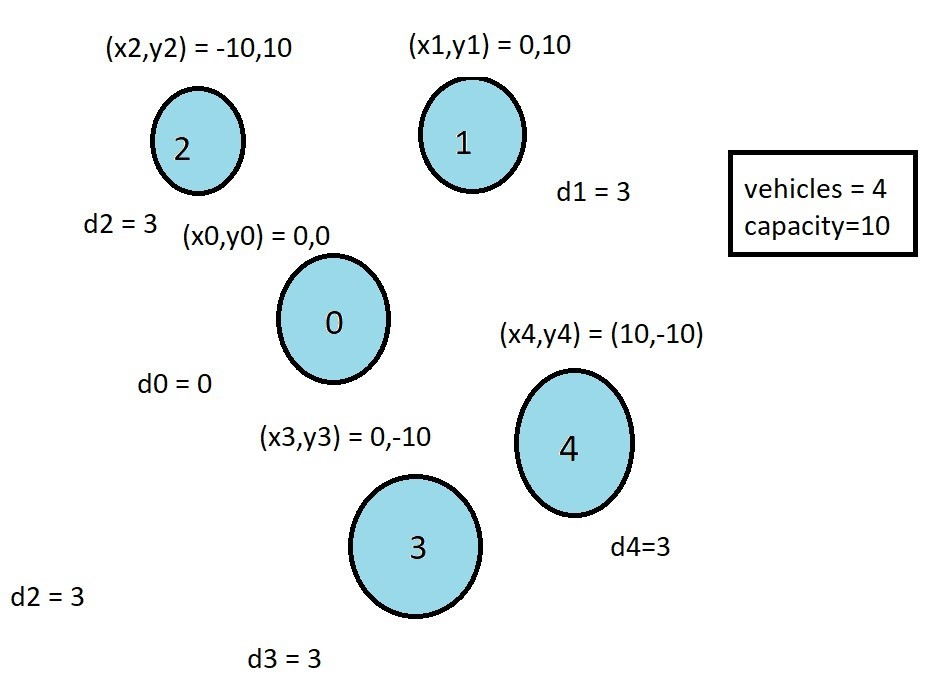
\includegraphics[width=1\linewidth]{
opti_1.jpg}\par  


Let’s solve the vehicle routing problem with simultaneous pick-up and delivery. Here we give some additional  inputs to the computerized VRPPD algorithms  then we get additional output.

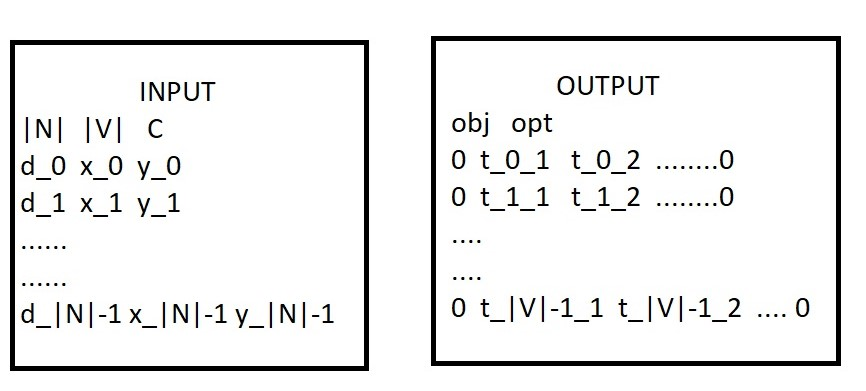
\includegraphics[width=1\linewidth]{
opti_2.jpg}\par  


In our first tour The minimum cost is 80.6. Here vehicle 1 is denoted using green  lines and vehicle 2  path is denoted with purple color. Here the main constrain is that every demand should be less than the total capacity of the vehicle and also demand should satisfy one's. we have given the sequence of deliveries of vehicle i is denoted  using Ti\\
\\
Path of vehicle 1 (T1) : 0 → 1 → 2 → 3 → 0 \\
Path of vehicle 2 (T2) : 0 → 4 → 0 \\

\begin{center}
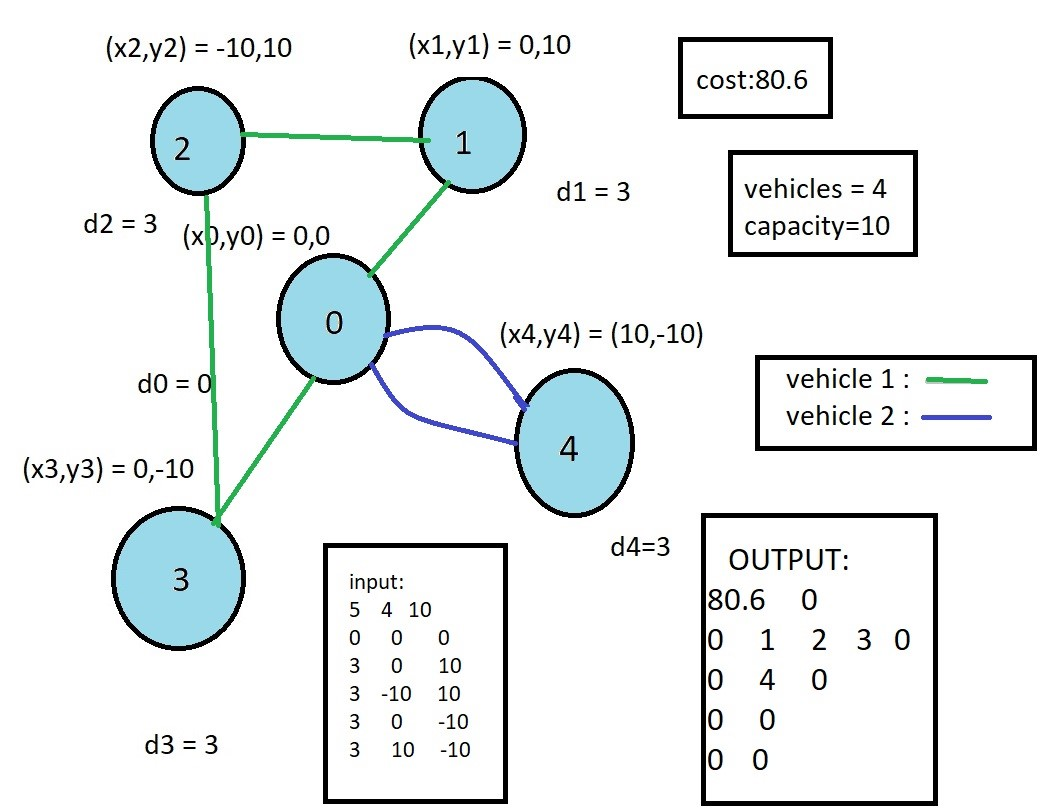
\includegraphics[width=1\linewidth]{
opti_3.jpg}\par  
\end{center}
\vspace{5}

In the second interaction we minimize our cost and it is better than the previous one.hear we get minimum cost is 68.3 which is optimizing value compare to  previous one.\\
\vspace{5}
\begin{center}
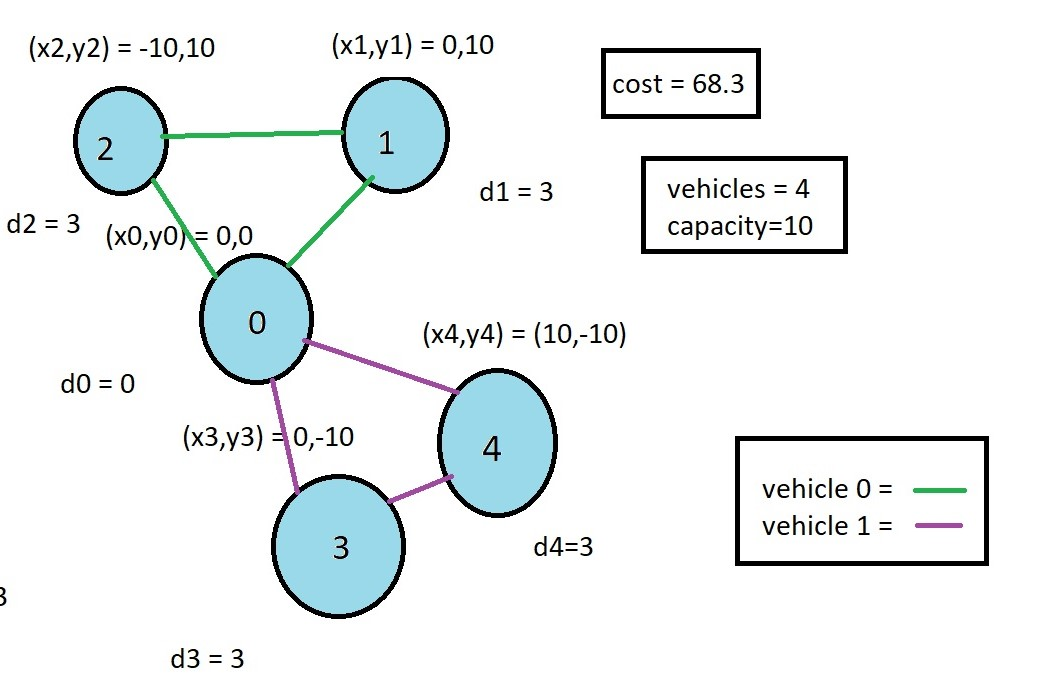
\includegraphics[width=1\linewidth]{
opti_4.jpg}\par  
\end{center}
Path of vehicle 0 (T0) : 0 → 1 → 2 → 0\\
Path of vehicle 1 (T1) : 0 → 4 → 3 → 0\\

\section{{\textbf{CONCLUSION}}}
In this paper, we have considered the Vehicle Routing Problem for pickup and delivery problem (PDP). For solving the problem, we generated the LPP for the graph. Then by using the Routing Index Manager, we solved the problem. The advantage of this method is that modern vehicle routing tools use machine learning-based solutions, which are used to increase efficiency and reduce fuel costs. We also developed code for solving these types of problems in PyCharm. The problem for finding the complexity is an NP-complete problem.\\ 
Our computations show that this problem can also be converted into a Distribution Problem. This problem has many several variations, which are divided using different constraints like capacity of the vehicle, length of route and repair time, delivery of products, and time of assortment. But here we will consider only the problem of Pickup and Deliveries of goods using vehicles and try to minimize the total cost of transport. Many modifications can be made in our problem to solve several problems in real life.


\section{{\textbf{ACKNOWLEDGMENT}}}
We are thankful to Prof. Manish Kumar for providing us the opportunity to research on such topics and have the experience of applying what we study to real-life scenarios. Also thankful to TAs for guiding us throughout the semester to carry out our research in the correct direction.









\begin{thebibliography}{00}
\bibitem{} \url{https://www.researchgate.net/profile/Ashima-Gupta-5/publication/327192553/figure/fig1/AS:703224415805440@1544673174324/Classical-Vehicle-Routing-problem.png }  \\

\bibitem{} \url{F. A. Tang Montané and R. D. Galvão, “A tabu search algorithm for the vehicle routing problem with simultaneous pick-up and delivery service,” Computers & Operations Research, vol. 33, no. 3, pp. 595–619, 2006}   \\
\bibitem{} \url{https://www.researchgate.net/figure/Classical-Vehicle-Routing-problem_fig1_327192553}   \\

\bibitem{} \url{K. Fleszar, I. H. Osman, and K. S. Hindi, “A variable neighbourhood search algorithm for the open vehicle routing problem,” European Journal of Operational Research, vol. 195, no. 3, pp. 803–809, 2009.}   \\
\bibitem{} \url{H. Hernández-Pérez and J.-J. Salazar-González, “A branch-and-cut algorithm for a traveling salesman problem with pick-up and delivery,” Discrete Applied Mathematics, vol. 145, no. 1, pp. 126–139, 2004} \\
\bibitem{} \url{http://www.scielo.org.co/scielo.php?script=sci_arttext&pid=S1909-24742016000100021#f1 } \\

\bibitem{} \url{S. Kirkpatrick, C. D. Gelatt,, Jr., and M. P. Vecchi, “Optimization by simulated annealing,” Science, vol. 220, no. 4598, pp. 671–680, 1983.}   \\
\bibitem{} \url{https://link.springer.com/article/10.1007/s10479-017-2722-x#Sec3  } \\


\bibitem{} \url{Beck, J.C.; Prosser, P.; Selensky, E. (2003). "Vehicle routing and job shop scheduling: What's the difference?" (PDF). Proceedings of the 13th International Conference on Artificial Intelligence Planning and Scheduling}   \\
\bibitem{} \url{https://neo.lcc.uma.es/vrp/vrp-instances/  } \\

\bibitem{} \url{https://core.ac.uk/download/19477982.pdf}\\
\bibitem{} \url{https://en.wikipedia.org/wiki/Vehicle_routing_problem}\\

\bibitem{} \url{G. Mosheiov, “Vehicle routing with pick-up and delivery: tour-partitioning heuristics,” Computers & Industrial Engineering, vol. 34, no. 3, pp. 669–684, 1998.}   \\
\bibitem{} \url{ http://webpages.ull.es/users/hhperez/PDsite/index.html.}   \\
\end{thebibliography}  

\vspace{12pt}

\section{{\textbf{APPENDIX}}}
\begin{center}
    

\subsection{\textbf{Input}}    
\begin{center}
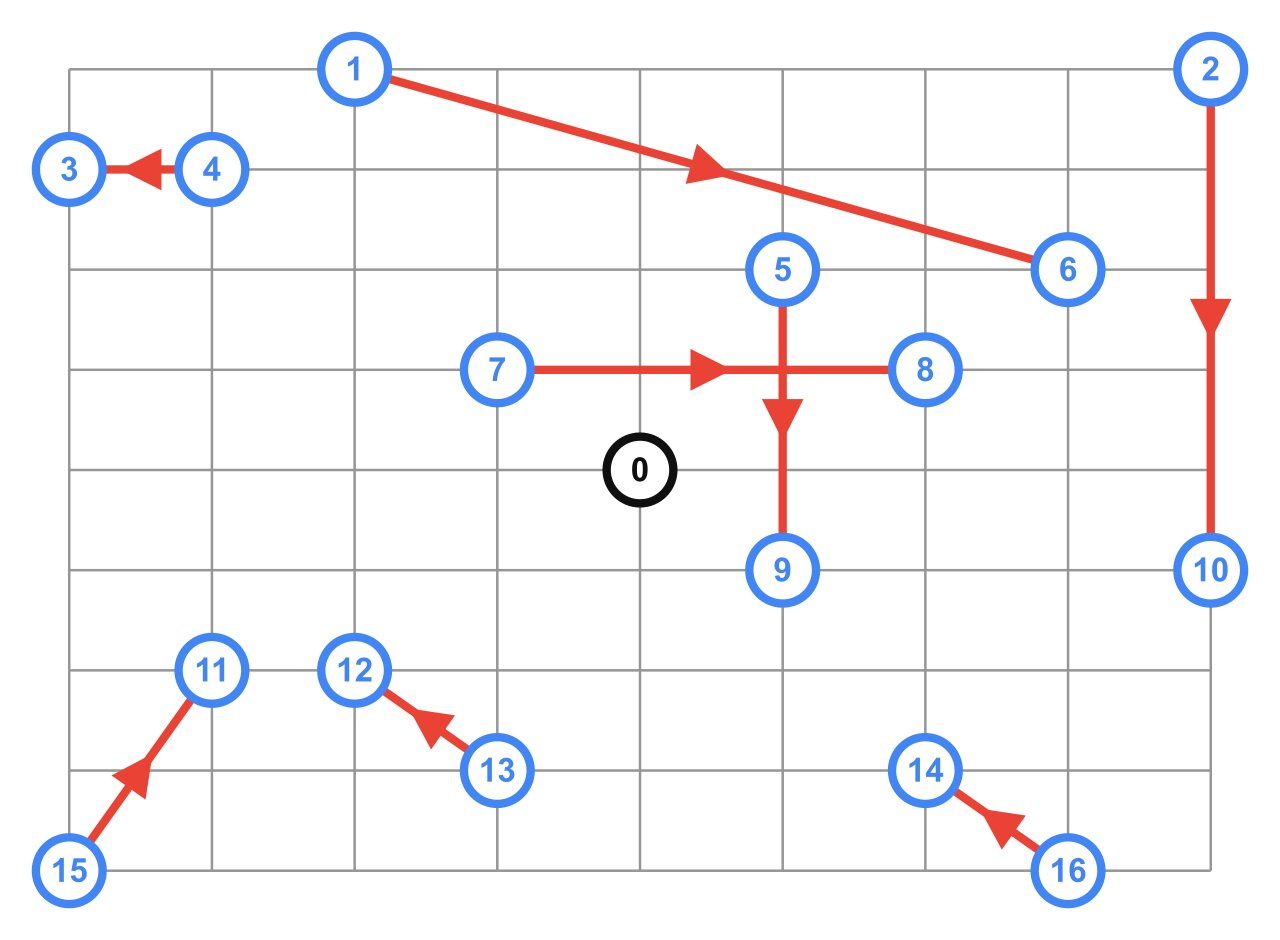
\includegraphics[width=1\linewidth]{
input.jpg}\par  
\end{center}

\begin{center}
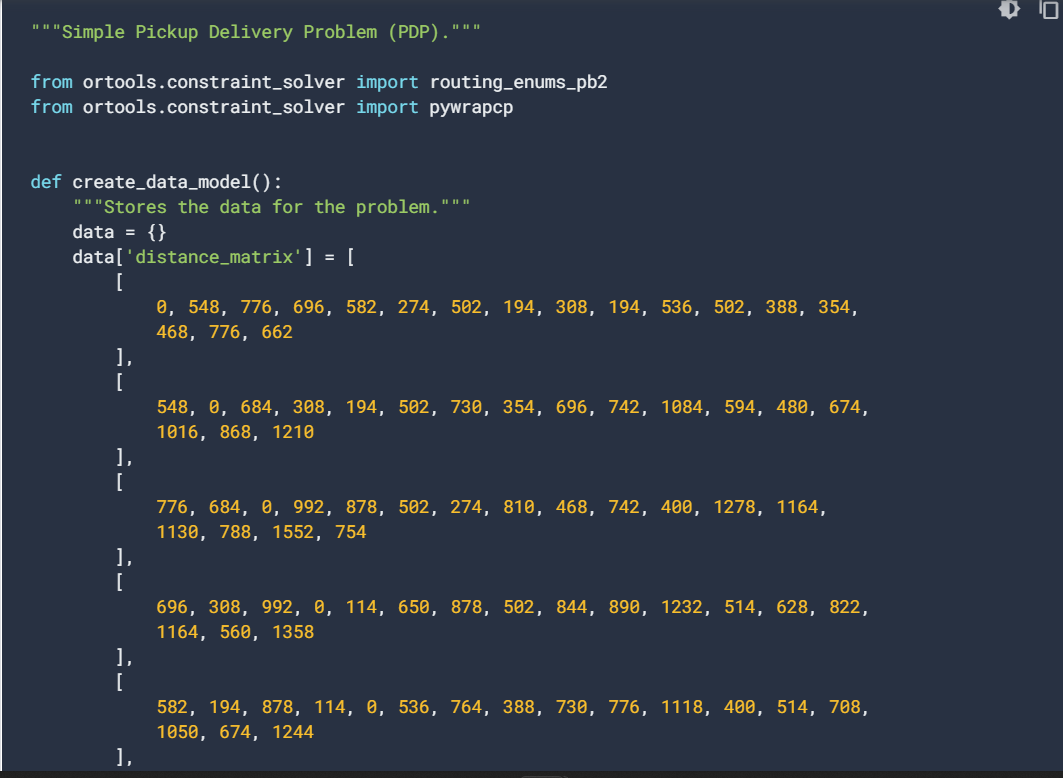
\includegraphics[width=1\linewidth]{
1.png}\par  
\end{center}

\begin{center}
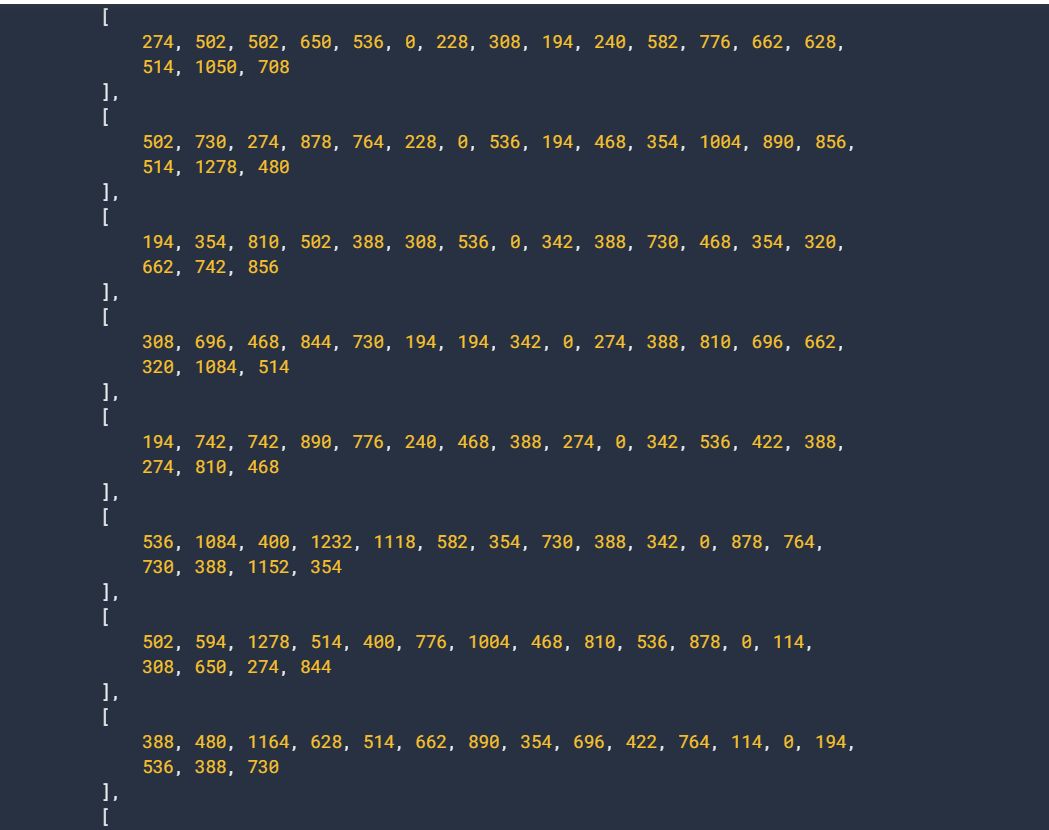
\includegraphics[width=1\linewidth]{
2.png}\par  
\end{center}

\begin{center}
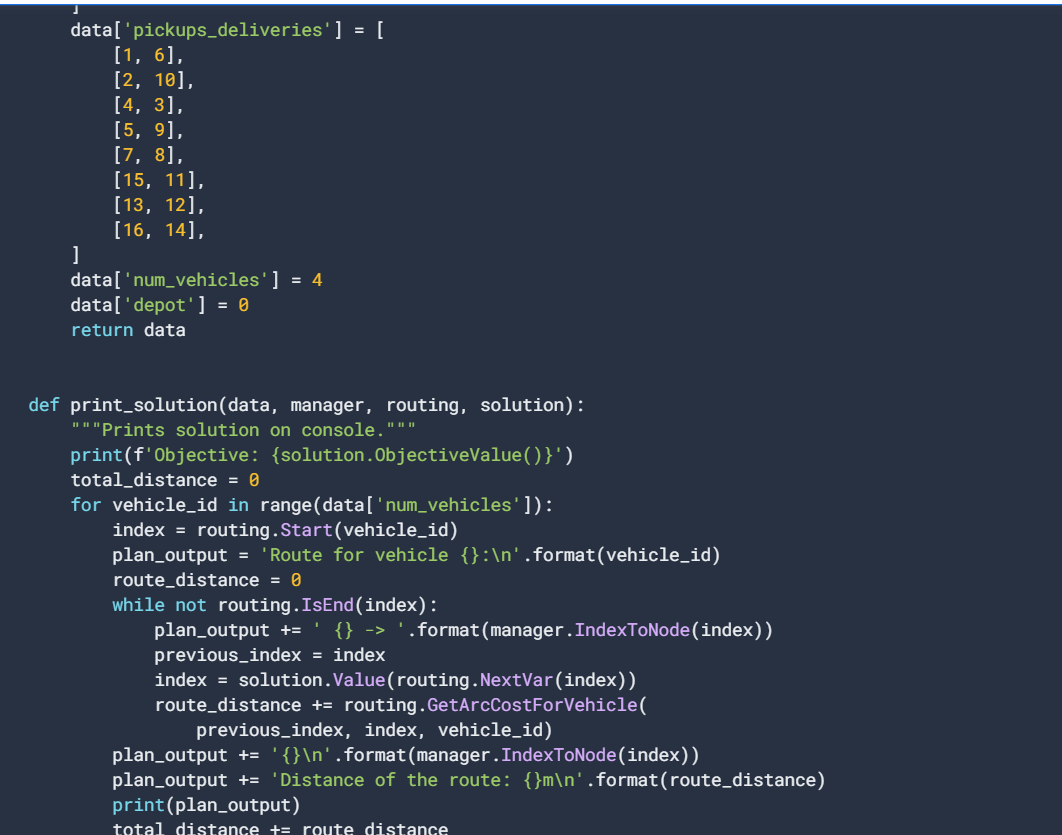
\includegraphics[width=1\linewidth]{
3.png}\par  
\end{center}
\subsection{\textbf{Main code}}  
\begin{center}
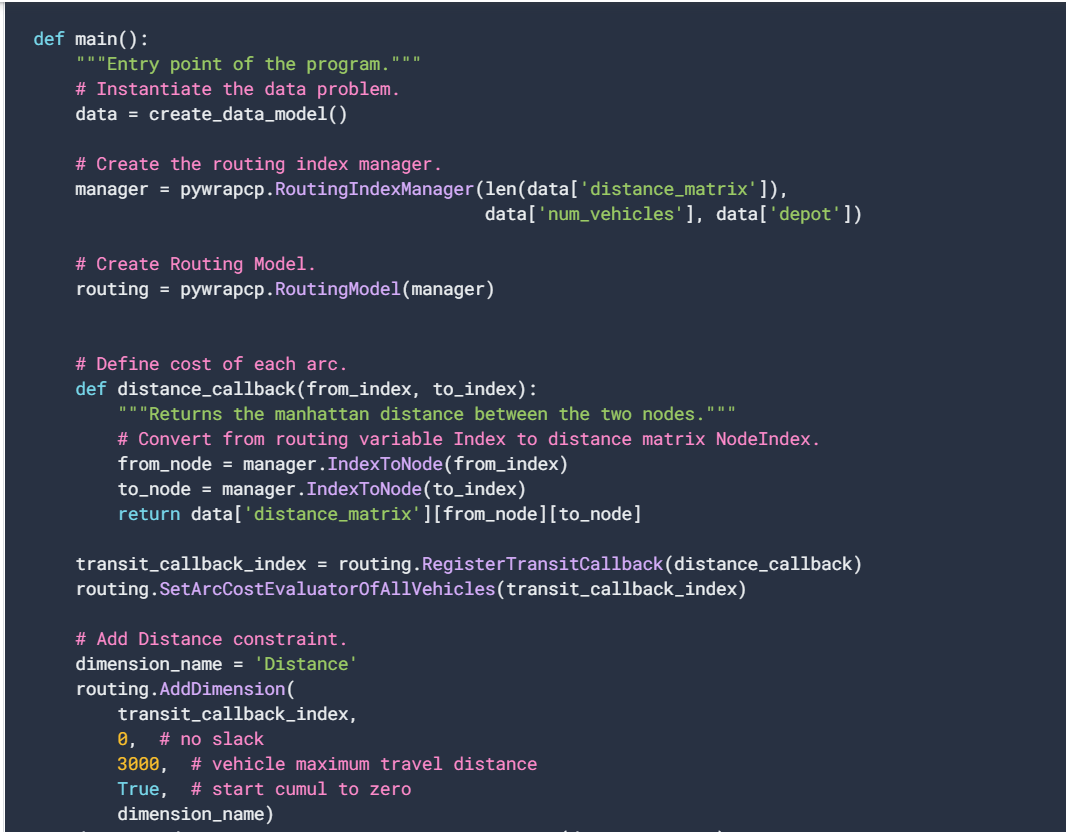
\includegraphics[width=1\linewidth]{
4.png}\par  
\end{center}

  
\begin{center}
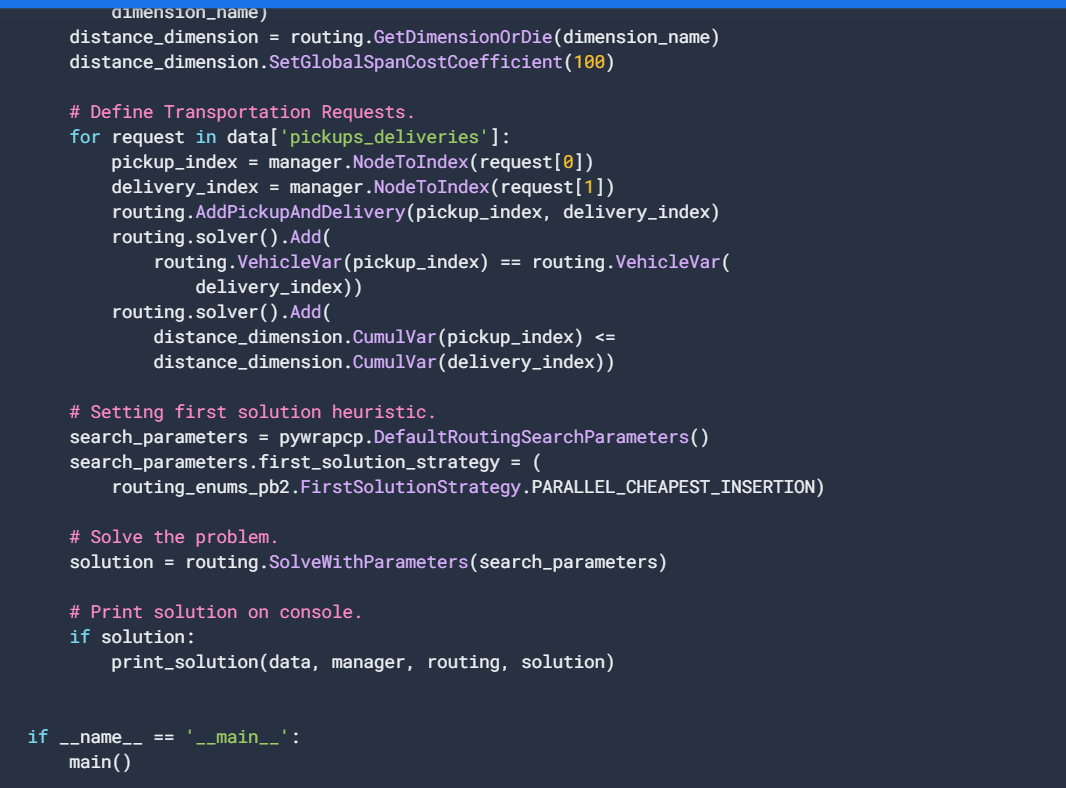
\includegraphics[width=1\linewidth]{
5.png}\par  
\end{center}

\subsection{\textbf{Output}}    
\begin{center}
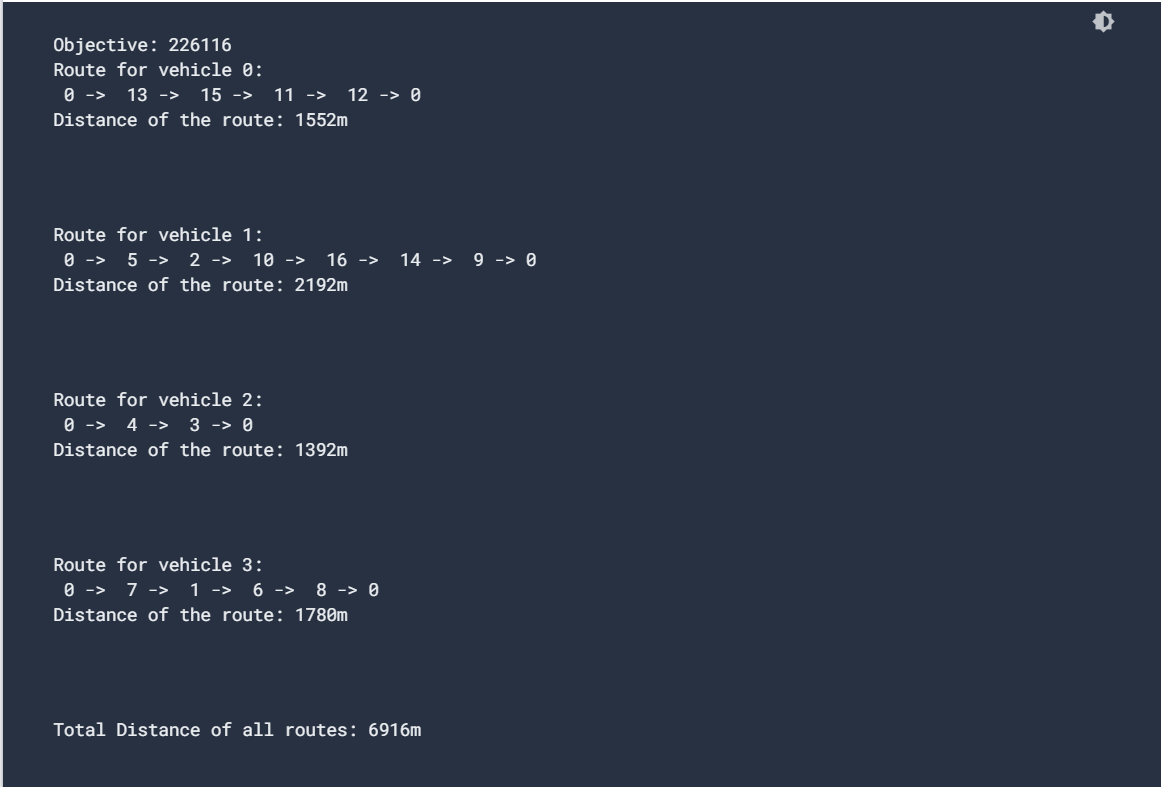
\includegraphics[width=1\linewidth]{
result.png}\par  
\end{center}

\begin{center}
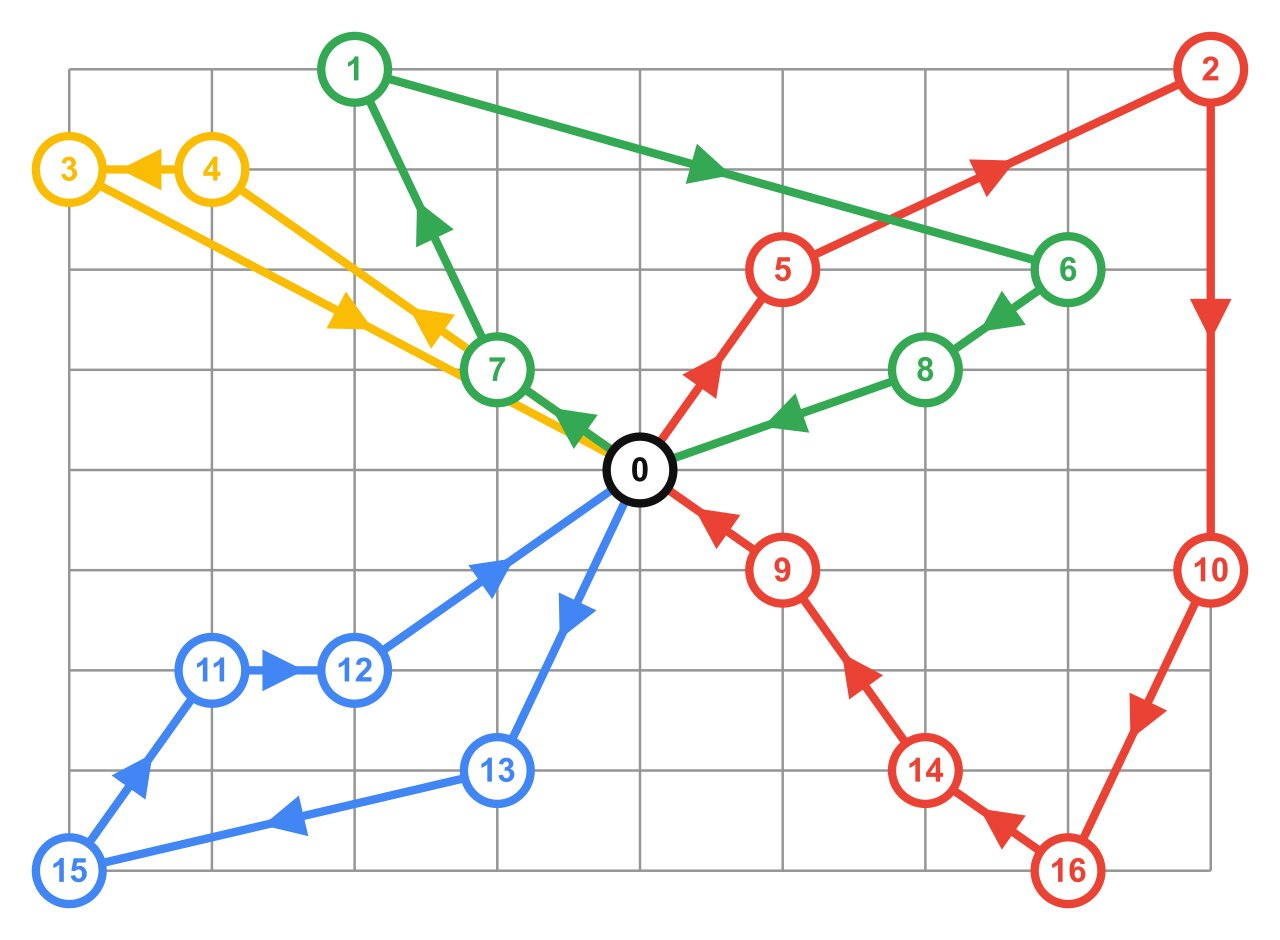
\includegraphics[width=1\linewidth]{
output.jpg}\par  
\end{center}


\subsection{\textbf{solution Code link}}    

\href{https://bit.ly/3r7MkHB}{Code}
\end{center}
\end{document}
